\section{Python : origine et philosophie}
\subsection{L'origine de Python}
\begin{frame}
  \frametitle{L'origine de Python}
  \begin{columns}
    \begin{column}{5cm}
      \begin{itemize}
        \item<1-> Apparition en 1991
        \item<2-> Créé par Guido van Rossum
        \item<3-> Nombreuses références aux Monty Python
      \end{itemize}
    \end{column}
    \begin{column}{5cm}
      \begin{overprint}
        \includegraphics<2>[scale=0.04]{guido.jpg}
        \includegraphics<3>[scale=0.15]{spam.jpg}
      \end{overprint}
    \end{column}
  \end{columns}
\end{frame}

\subsection{Valeurs et philosophie}
\begin{frame}
\frametitle{Valeurs et philosophie}
  % En fait ici on présente ce qu'on va voir, afin de pouvoir terminer par CQFD!
  \begin{itemize}
    \item Orienté objet
    %note feth:
    %utilisation souple (programmation impérative, orientée aspect, haut niveau ou bas niveau...)
    \pause
    \item Extensible (librairies standard, modules C, C++, \ldots)
  \end{itemize}
\end{frame}

\subsection{La recherche du meilleur chemin}
\begin{frame}
\frametitle{La recherche du meilleur chemin}
  \begin{itemize}
    \item Un travail de recherche via les PEP
    \pause
    %note feth:
    %mots clefs: efficacité en terme de lisibilité, pythonique, élégance (comme en maths)
    \item 1 seul bon moyen de faire
  \end{itemize}
\end{frame}



\section{IPython, le Python interactif}
\subsection{Les fonctionnalités}

\begin{frame}
  \frametitle{Fonctionnalités}
  \begin{itemize}
    \item Exécution de code dynamique
    \item Interaction avec le système
    \item Historique des commandes
    \item Journalisation
  \end{itemize}
\end{frame}

\subsection{Utile pour \ldots}
\begin{frame}[fragile]
  \frametitle{Utile pour \ldots}
    \begin{itemize}
      \item apprendre la syntaxe
    \end{itemize}
  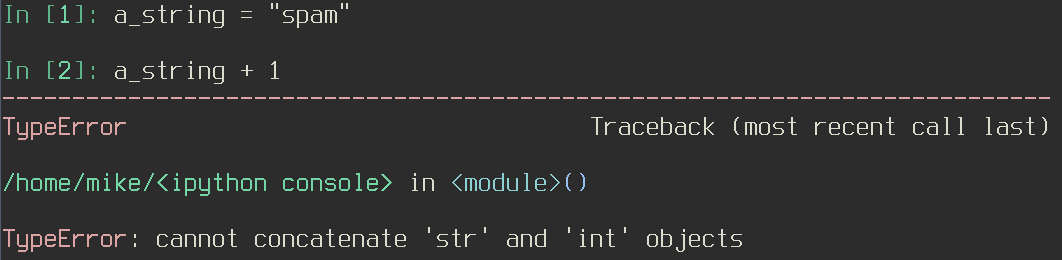
\includegraphics[scale=0.35]{apprendre.png}

\end{frame}

\begin{frame}
  \frametitle{Utile pour \ldots}
    \begin{itemize}
      \item prototyper une fonctionnalité
    \end{itemize}
    %note feth:
    % 1)
    %plutôt qu'un getter sur une var publique
    %je suggère une fonction qui fasse quelque chose, comme
    %def greet(self, name):
    %    return "%s greets %s." (self.name, name)
    % à votre avis ?
    %
    % 2) mentionner le ducktyping ? (à votre avis)
    % 2.1) Pour être callable il suffit d'implémenter 'def \_\_call\_\_(...)'
    % 2.2) pour être indexable : \_\_setitem\_\_(...), \_\_getitem\_\_(...)
    % Je ne sais pas trop comment insérer ça dans le cours, ça devrait venir plus tard dans le détail et c'est un peu hors sujet dans le prototypage..
  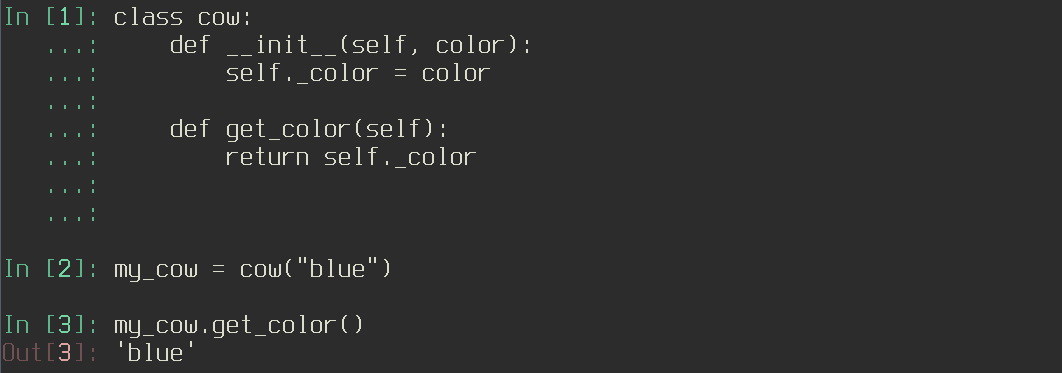
\includegraphics[scale=0.35]{prototype.png}
\end{frame}

\begin{frame}
  \frametitle{Utile pour \ldots}
    \begin{itemize}
      \item la découverte interactive d'une API
    \end{itemize}
  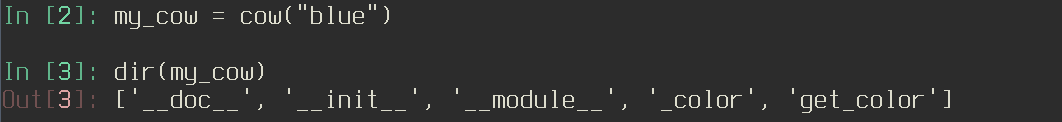
\includegraphics[scale=0.35]{api_discover.png}
\end{frame}

\begin{frame}
  \frametitle{Utile pour \ldots}
    \begin{itemize}
      \item embarquer un shell IPython dans ses programmes
    \end{itemize}
  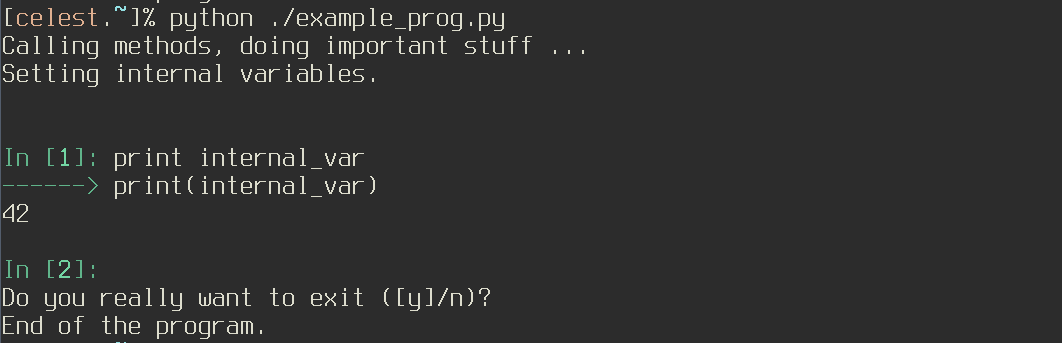
\includegraphics[scale=0.35]{embedded_ipython.png}
\end{frame}

\section{Les types de base de Python}
\subsection{Quelques types simples}
% 1 Les types de base Python
% 1.1 Quelques types simples
%     - entiers
%     - flottants
%     - True, False
%     - None

\begin{frame}
  \frametitle{Quelques types simples}
  \begin{itemize}
    \item<1-> les entiers
    \item<2-> les flottants
    \item<3-> les booléens
    \item<4-> la valeur 'Rien'
  \end{itemize}
\end{frame}

\begin{frame}
  \frametitle{Quelques types simples}
    \begin{itemize}
      \item les entiers
    \end{itemize}
    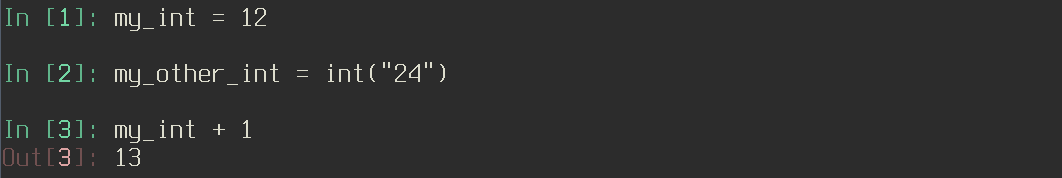
\includegraphics[scale=0.35]{type_int.png}
\end{frame}

\begin{frame}
  \frametitle{Quelques types simples}
    \begin{itemize}
      \item les flottants
    \end{itemize}
XXX TODO
\end{frame}

\begin{frame}
  \frametitle{Quelques types simples}
    \begin{itemize}
      \item les booléens : \alert{True, False}
      \item la valeur 'Rien' : \alert{None}
    \end{itemize}
XXX TODO
\end{frame}

% 1.2 Quelques structures de données
%     - les chaines de caractère sont des séquences comme les autres
%     - séquence: list modifiable, tuple non modifiable, queue...
%     - dictionnaire
%     - ensemble (partie gauche d'un dict): set modifiable, frozenset non modifiable

\subsection{Quelques structures de données}
\begin{frame}
  \frametitle{Quelques structures de données}
  \begin{itemize}
      \item<1-> les chaînes de caractère, un cas particulier de séquence
      \item<2-> les autres séquences : tuples, listes, queue, \ldots
      \item<3-> les dictionnaires
      \item<4-> les sets, frozenset
    \end{itemize}
\end{frame}

\begin{frame}
  \frametitle{Quelques structures de données}
    \begin{itemize}
      \item les chaînes de caractères
    \end{itemize}
    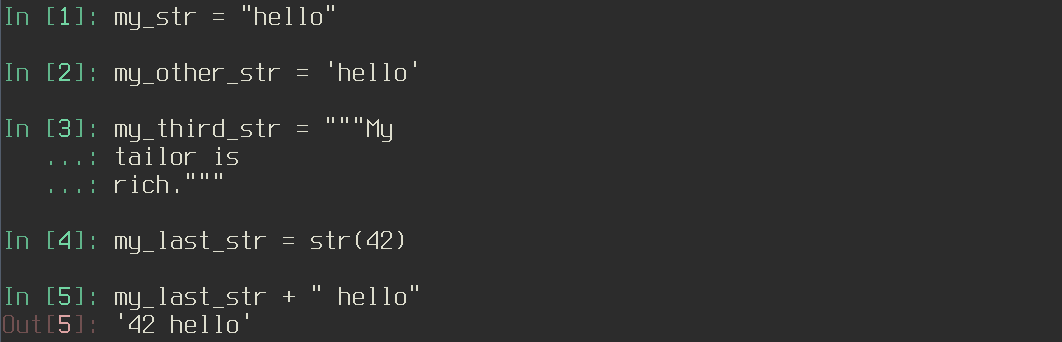
\includegraphics[scale=0.35]{type_str.png}
\end{frame}

\begin{frame}
  \frametitle{Quelques structures de données}
    \begin{itemize}
      \item les tuples
    \end{itemize}
    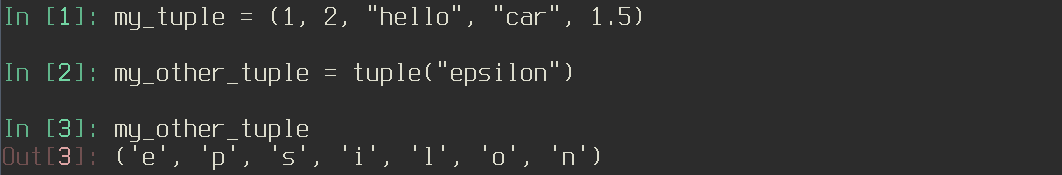
\includegraphics[scale=0.35]{type_tuple.png}
\end{frame}

\begin{frame}
  \frametitle{Quelques structures de données}
    \begin{itemize}
      \item les listes
    \end{itemize}
    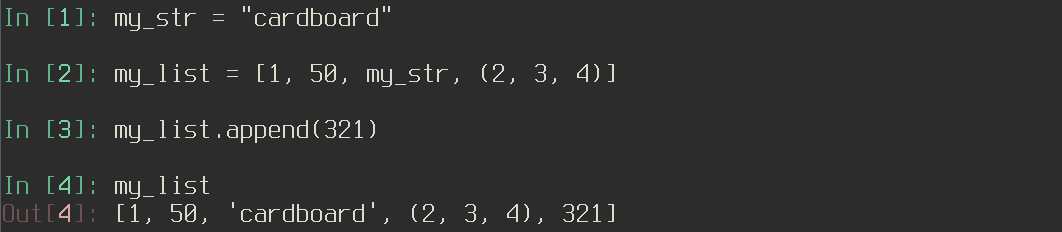
\includegraphics[scale=0.35]{type_list.png}
\end{frame}

\begin{frame}
  \frametitle{Quelques structures de données}
    \begin{itemize}
      \item les dictionnaires
    \end{itemize}
    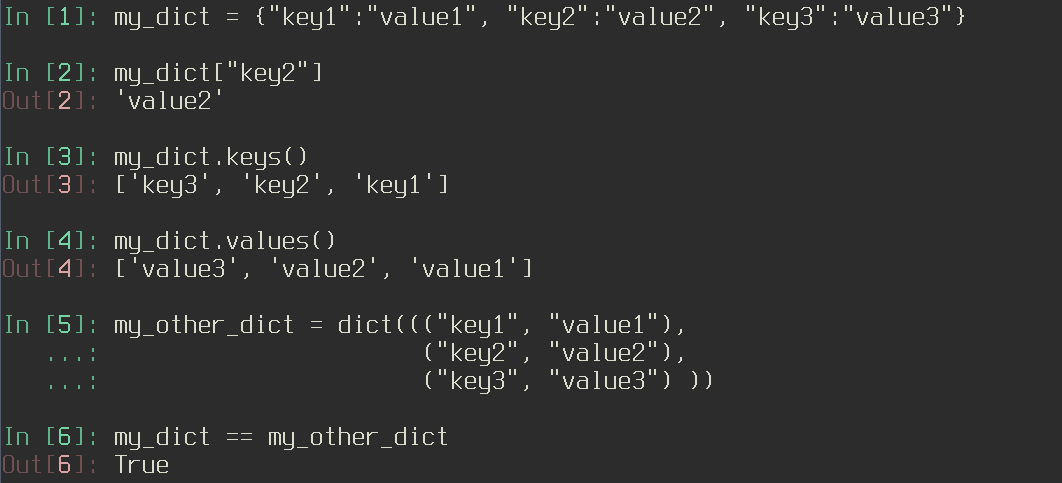
\includegraphics[scale=0.35]{type_dict.png}
\end{frame}

\begin{frame}
  \frametitle{Quelques structures de données}
    \begin{itemize}
      \item les sets
    \end{itemize}
    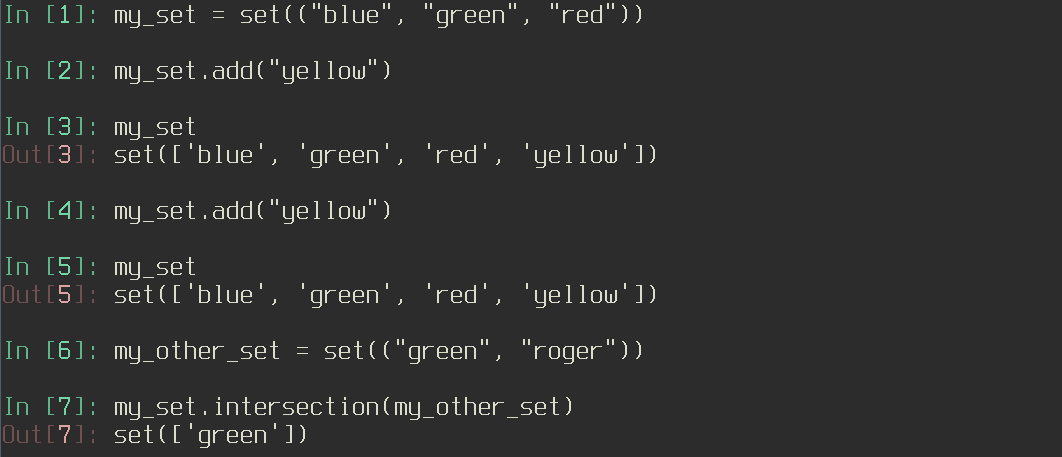
\includegraphics[scale=0.35]{type_set.png}
\end{frame}

% 1.3 Quelques autres types courants (juste les évoquer)
%     - classe, fonction ou méthode, module...

\subsection{Quelques autres types courants}
\begin{frame}
  \frametitle{Quelques autres types courants}
    \begin{itemize}
      \item les classes
      \item les fonctions/méthodes
      \item les modules
    \end{itemize}
\end{frame}

% 2 La syntaxe de Python
% 2.1 instructions
%     - séparateur d'instruction : ';' (éviter) ou '\\n'
% 2.2 blocs
%     - contexte (scope) défini par bloc
%     - blocs définis par :
%       - leur niveau d'indentation
%       - bloc de niveau inférieur suit une ligne
%         - qui commence par un mot clef (if, while, for, def, class, with)
%         - se termine par ':'
% et continuer comme julien l'a fait sur if etc.
% Ce point 2.2 est une introduction aux différents blocs qu'on va traiter ensuite.

\section{La syntaxe de Python}

\subsection{Les instructions}
\begin{frame}
  \frametitle{Les instructions}
XXX TODO
  \semiverbatim{séparateur d'instruction : ';' (éviter) ou '\\n'}
\end{frame}

\subsection{Les blocs}
\begin{frame}[fragile]
  \frametitle{Les blocs}
XXX TODO
  \begin{verbatim}
- contexte (scope) défini par bloc
- blocs définis par :
  - leur niveau d'indentation
  - bloc de niveau inférieur suit une ligne
    - qui commence par un mot clef (if, while, for, def,
      class, with)
    - se termine par ':'
  \end{verbatim}

\end{frame}

\subsection{Les déclarations conditionnelles}
\begin{frame}[fragile]
  \frametitle{Syntaxe de base}
  \begin{lstlisting}
if condition1:
    declaration1
elif condition2:
    declaration2
else:
    declaration3
  \end{lstlisting}
\end{frame}

\begin{frame}[fragile]
  \frametitle{Structure de base - exemple}
  \begin{lstlisting}
my_str = "word"
if 1 > 2:
    print "1>2"
elif my_str == "word":
    print "my_str = word"
else:
    print "else"
  \end{lstlisting}

  \begin{beamercolorbox}{terminal}
  \begin{semiverbatim}
 \$ python example.py
 \uncover<2>{my_str = word} \end{semiverbatim}
  \end{beamercolorbox}

\end{frame}

\begin{frame}[fragile]
  \frametitle{Les conditions}
  \begin{itemize}
    \item les comparaisons
  \end{itemize}
  \begin{beamercolorbox}{terminal}
  \begin{semiverbatim}
\uncover<1->{ In [1]: (1 == 2, 1 < 2, 2 < 1, 1 != 2)}
\uncover<1->{ Out[1]: (False, True, False, True)}

\uncover<2>{ In [2]: my_str = "hello"}
\uncover<2>{ In [2]: (my_str == "hello", my_str > "helln",
    ...: my_str < "hellq")}
\uncover<2>{ Out[2]: (True, True, True)}\end{semiverbatim}
    \end{beamercolorbox}
\end{frame}

\begin{frame}[fragile]
  \frametitle{Les conditions}
  \begin{itemize}
    \item les opérateurs booléens
  \end{itemize}
  \begin{beamercolorbox}{terminal}
  \begin{semiverbatim}
 In [1]: not True and False or not False
 Out[1]: True\end{semiverbatim}
  \end{beamercolorbox}
\end{frame}

\begin{frame}[fragile]
  \frametitle{Les conditions}
  \begin{itemize}
    \item par extension, certains objets vides sont équivalent à False
  \end{itemize}
  \begin{beamercolorbox}{terminal}
  \begin{semiverbatim}
 In [1]: my_str = ""
 In [1]: if not my_str:
    ...:     print "False"
 False\end{semiverbatim}
  \end{beamercolorbox}
\end{frame}

\subsection{Les boucles}
\begin{frame}[fragile]
  \frametitle{Syntaxe de for}
  \begin{lstlisting}
for item in <generator>:
    code ...
  \end{lstlisting}
\end{frame}

\subsection{Les méthodes/functions}
\begin{frame}[fragile]
\end{frame}

\subsection{Les classes}
\begin{frame}[fragile]
\end{frame}

\section{Quelques librairies standard}
\begin{frame}[fragile]
\end{frame}

%  \framesubtitle{The proof uses \textit{reductio ad absurdum}.}
%  \begin{theorem}
%      There is no largest prime number.
%  \end{theorem}
%  \begin{proof}
%    \begin{enumerate}
%      \item<1-| alert@1> Suppose $p$ were the largest prime number.
%      \item<2-> Let $q$ be the product of the first $p$ numbers.
%      \item<3-> Then $q+1$ is not divisible by any of them.
%      \item<1-> Thus $q+1$ is also prime and greater than $p$.\qedhere
%    \end{enumerate}
%  \end{proof}

%\setbeamercolor{terminal}{fg=white, bg=black}
%\begin{beamercolorbox}{terminal}
%\end{beamercolorbox}
